% ============================================================
\chapter{Vectors, Data, and Linear Structure}
\label{ch:vectors-data}
% ============================================================

\section*{Chapter Preview}
\addcontentsline{toc}{section}{Chapter Preview}

The word ``vector'' does not mean only an arrow in the plane. In linear
algebra, a vector is any object that belongs to a space where addition and
scalar multiplication make sense. A signal, a polynomial, an image, a list of
features, and an arrow in $\R^3$ can all be vectors.

\section{Mathematics as a Productive Language}

Mathematics is not only a descriptive language. A descriptive language names
things. A productive language lets us compute with them, transform them, and
derive new facts. Linear algebra is productive because it gives a common
language for many different-looking objects.

The same operation may appear in several forms:

\begin{itemize}
  \item adding arrows in the plane,
  \item adding coefficient lists of polynomials,
  \item adding signals pointwise,
  \item adding image arrays pixel by pixel,
  \item adding feature vectors in a data set.
\end{itemize}

The objects look different. The structure is the same.

\begin{figure}[h]
  \centering
  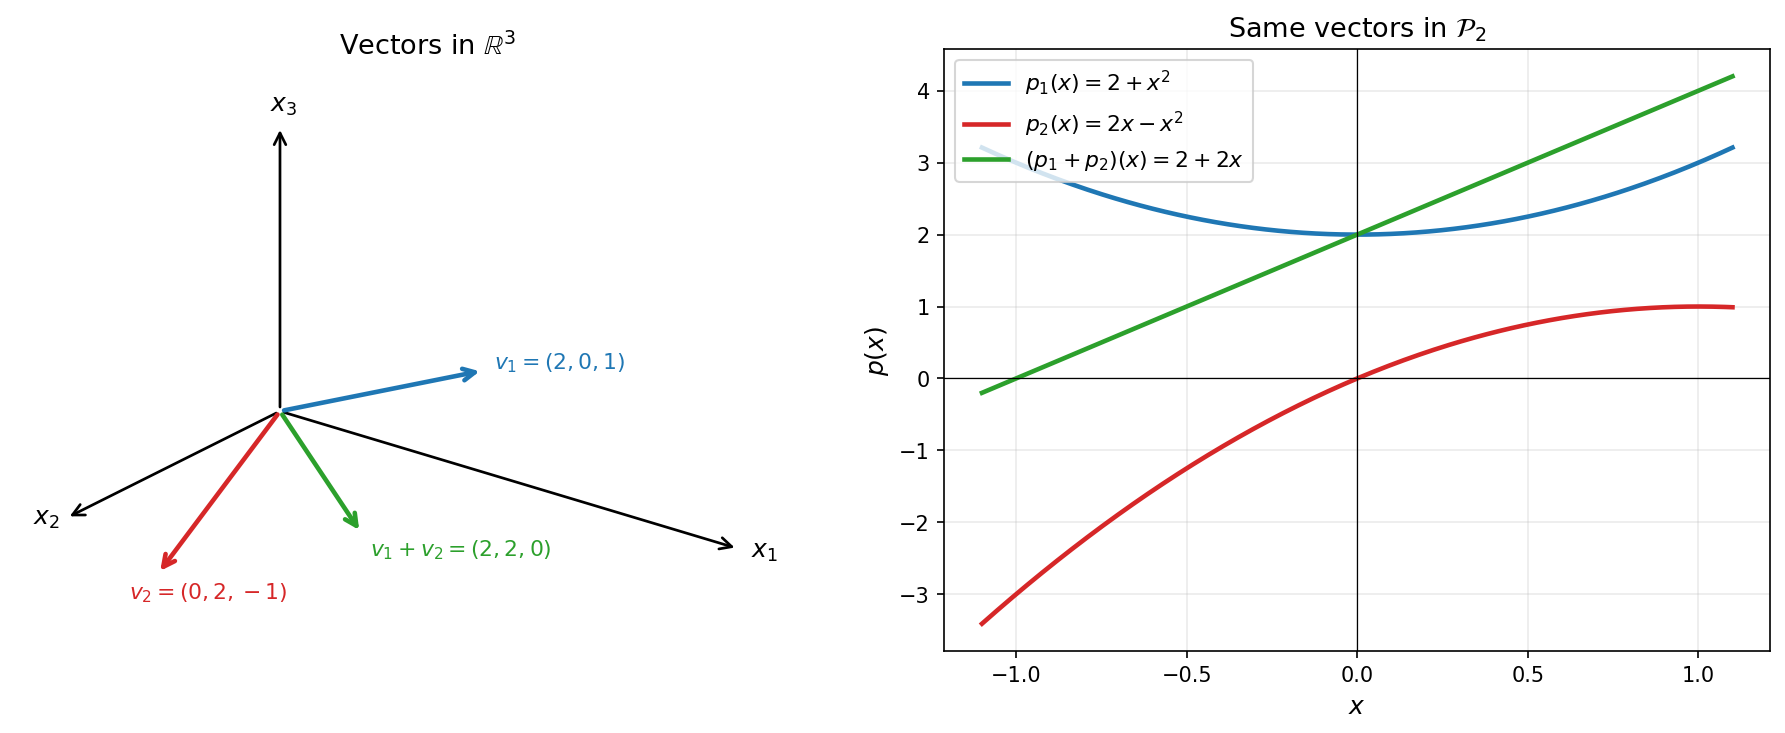
\includegraphics[width=\textwidth]{book/assets/figures/core/fig01_vectors.png}
  \caption{The same vector-space operation in two concrete settings:
  arrows in space and polynomials represented by coefficients.}
\end{figure}

\begin{remark}[Two legs of the subject]
Practical linear algebra has two legs. One leg is computation: implementation,
experiments, data, and numerical algorithms. The other is theory: definitions,
proofs, invariants, and guarantees. Either leg by itself is unstable. The book
will keep switching between them.
\end{remark}

\begin{definition}
  A \emph{scalar} is a number used to scale vectors. In this book the scalars
  usually come from $\R$, and sometimes from $\C$.
\end{definition}

\begin{definition}
  A \emph{vector} is an element of a vector space.
\end{definition}

This definition is intentionally circular until vector spaces are defined in
Chapter~\ref{ch:vector-spaces-subspaces}. The important point for now is that a
vector is not defined by what it looks like. It is defined by the operations it
supports.

\section{Fields of Scalars}

The scalars in a vector space come from a field. A field is a number system
where addition, subtraction, multiplication, and division by nonzero elements
behave as expected. The main examples are $\R$ and $\C$.

\begin{example}[The field $\Z_2$]
The set $\Z_2=\{0,1\}$ with arithmetic modulo $2$ is a field:
\[
  1+1=0,\qquad 1\cdot 1=1.
\]
It is useful for switches, parity checks, and error-correcting codes. This is
a reminder that linear algebra is not restricted to real numbers.
\end{example}

Over $\Z_2$, addition is the same as XOR. This small field will return in the
optional Hamming-code project, where a matrix detects and corrects one-bit
errors.

\section{Data as Vectors}

A grayscale image with $m$ rows and $n$ columns is an $m\times n$ array of
numbers. We may keep it as a matrix, or stack its entries into one long vector
in $\R^{mn}$. A color image has three such arrays, one for each color channel.

A data table with $N$ observations and $d$ features is usually represented by
a matrix $X\in \R^{N\times d}$. Each row is a data point. Each column is a
feature. This is already linear algebra.

This is also the first place where notation matters. The same image can be
stored as a rectangular array or stacked into one long vector. The same
polynomial can be drawn as a curve or stored as a coefficient list. The
mathematical object and its representation are not identical.

\begin{aimlbox}
Feature vectors are one of the simplest bridges from linear algebra to machine
learning. A model often begins by turning an object into a vector of numbers.
Linear algebra then describes how those numbers are transformed, compared,
projected, compressed, and approximated.
\end{aimlbox}

\section{Python: Arrays as Representatives}

In \Python, a vector is often represented by a one-dimensional \NumPy array.
The array is not the mathematical vector itself; it is a coordinate
representation of that vector.

\begin{lstlisting}
import numpy as np

u = np.array([2.0, -1.0, 3.0])
v = np.array([0.5, 4.0, 1.0])

print("u + v =", u + v)
print("3u    =", 3 * u)
print("zero  =", np.zeros(3))
\end{lstlisting}

When we later change basis, the same vector may have a different coordinate
array. The object is the same; the description changes.

\section*{Chapter Summary}
\addcontentsline{toc}{section}{Chapter Summary}

\begin{itemize}
  \item Vectors are defined by structure, not appearance.
  \item Scalars usually come from $\R$ or $\C$, but other fields can appear.
  \item Data objects such as signals, images, and feature lists can be vectors.
  \item A \NumPy array is a coordinate representation of a vector.
\end{itemize}

\section*{Where This Appears Later}
\addcontentsline{toc}{section}{Where This Appears Later}

Chapter~\ref{ch:vector-spaces-subspaces} defines vector spaces formally.
Chapter~\ref{ch:span-bases-coordinates} explains coordinates and bases.
Chapter~\ref{ch:svd-pca-low-rank} returns to data matrices, PCA, and compression.

\begin{labbox}
Lab 1 turns the vector-space axioms into \Python checks and explores span,
subspaces, and polynomial coefficient vectors.
\end{labbox}

\section*{Exercises}
\addcontentsline{toc}{section}{Exercises}

\subsection*{A. Theory}

\begin{exercise}
\exerciseid{1.A1}
Explain why the averaging rule in the chapter is linear. Your answer should
check both addition and scalar multiplication.
\end{exercise}

\begin{exercise}
\exerciseid{1.A2}
Give an example of a rule on grid states that is not linear. State which part
of linearity fails.
\end{exercise}

\subsection*{B. By Hand}

\begin{exercise}
\exerciseid{1.B1}
Let $u=(1,0,0,0)$ on a four-cell circular grid. Apply the averaging rule
$(Tu)_j=(u_{j-1}+u_{j+1})/2$ once by hand.
\end{exercise}

\subsection*{C. Python / NumPy}

\begin{exercise}
\exerciseid{1.C1}
Use basic \Python\ and \NumPy\ to implement the averaging rule for vectors of
length $N$. Test that your function satisfies
\texttt{T(u + v) == T(u) + T(v)} up to numerical tolerance.
\end{exercise}

\subsection*{D. Challenge}

\begin{exercise}
\exerciseid{1.D1}
Find a nonzero vector on a four-cell circular grid that is unchanged by the
averaging rule.
\end{exercise}

